%!TEX root = ../beamer.tex
% background on genotype-phenotype maps
% folder name: GPmaps

\begin{frame}
\begin{block}{}
An organism can be viewed as a collection of relatively fine-grained \textbf{genes} that are interpreted into phenotypes. If there are interaction constraints among the full set of genes the organism can be viewed as relatively coarse-grained \textbf{gene regulatory network modules}. 
\end{block}
\begin{block}{}
\textbf{Genotype-phenotype maps} can be evaluated at various levels of organization  beginning with a model of the gene and extending from simple molecular to ecosystem-level phenotypes.
\end{block}
\begin{block}{}
Repeated evaluation of the input-output dynamics of genotype-phenotype mappings on any given characteristic time-scale induces a \textbf{probability distribution over mappings} from \textbf{collections of genes} to \textbf{collections of phenotypes}. \textbf{Phenotypes} may be evaluated at any level, the level of evaluation determines the content of the collection of phenotype values.
\end{block}
\end{frame}
\begin{frame}
\begin{block}{\textbf{Question}}
For any genotype, given a \textbf{space of probability distributions}
on the \textbf{collection of possible genotype-phenotype maps}, does \textbf{modularization} over that genotype provide access to a \textbf{lesser}, \textbf{equivalent} or \textbf{greater} collection of correlations among the expression patterns of genes that define phenotypes?
\end{block}
\begin{block}{\textbf{Answer}}
For at least some forms of \textbf{modularization}, a \textbf{greater} collection of correlations among the expression patterns of genes is accessed via modularization.
\end{block}
\end{frame}

%\begin{frame}
\begin{block}{\textbf{Answer}}
For at least some forms of \textbf{modularization}, modularization provides access to a \textbf{greater} collection of correlations among the expression patterns of genes.
\end{block}
\end{frame}

\begin{frame}
\begin{center}
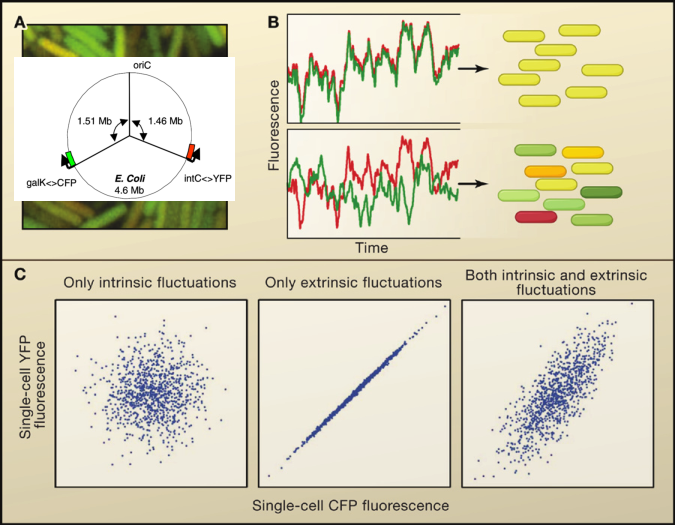
\includegraphics[width=0.8\textwidth]{fig/rajvOf1.pdf}\\
\hfill \cite{Raj2008a}
\end{center}
stochastic gene expression
\end{frame}

%!TEX root = ../../beamer.tex
\begin{frame}
\vspace{1em}
\frametitle{transcriptional bursting}
\begin{center}
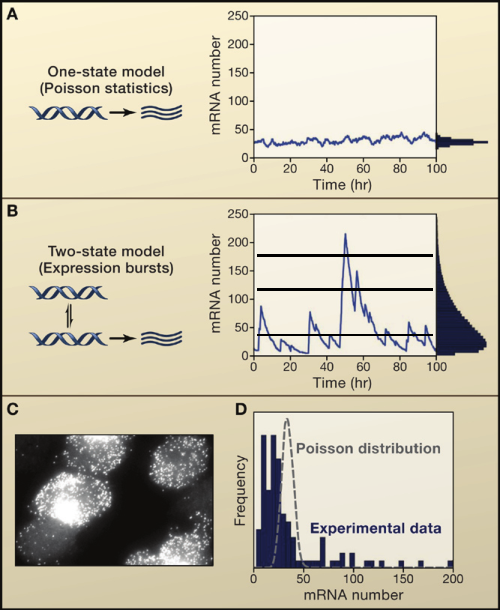
\includegraphics[width=0.5\textwidth]{fig/rajvOf3thresh.pdf}\\
\hfill \cite{Raj2008a}
\end{center}
\end{frame}

%!TEX root = ../../beamer.tex
\begin{frame}
\frametitle{stochasticity in gene expression}
\begin{center}
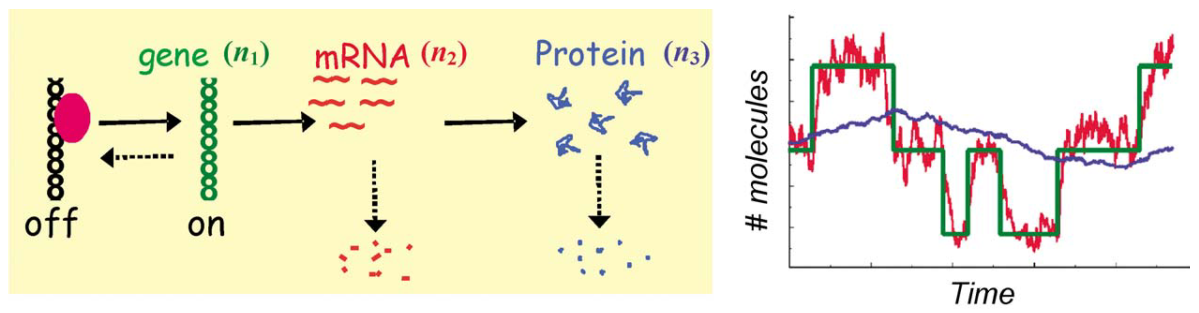
\includegraphics[width=0.9\textwidth]{fig/stochgeneexpdyn.png}\\
\end{center}
{\scriptsize
\begin{align*}
\text{gene activation } &n_1 \xrightarrow{\lambda_1^+ (n_1^{max}-n_1)}n_1+1\\
\text{gene inactivation } &n_1 \xrightarrow{\lambda_1^- n_1}n_1-1\\
\text{transcription } &n_2 \xrightarrow{\lambda_2 n_1}n_2+1\\
\text{mRNA degradation } &n_2 \xrightarrow{n_2/\tau_2}n_2-1\\
\text{translation } &n_3 \xrightarrow{\lambda_3 n_2}n_3+1\\
\text{proteolysis } &n_3 \xrightarrow{n_3/\tau_3}n_3-1
\end{align*}}\\
\hfill \cite{Paulsson2005}
\end{frame}


%!TEX root = ../../beamer.tex
\begin{frame}
\frametitle{stochasticity in gene expression}
\begin{center}
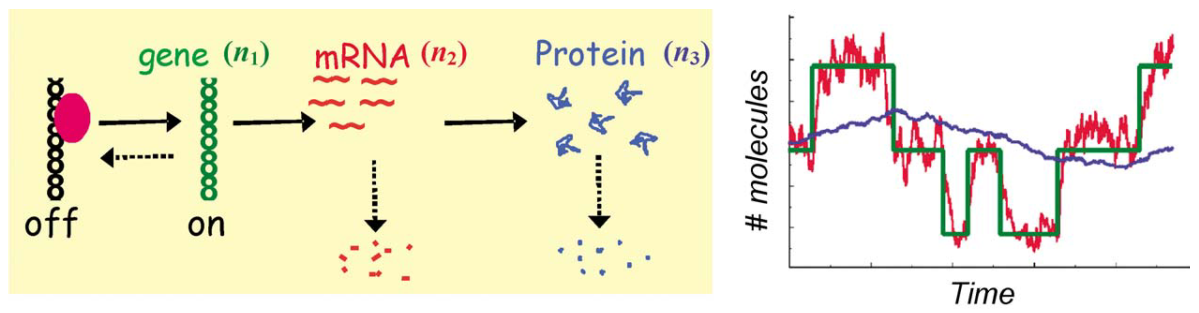
\includegraphics[width=0.9\textwidth]{fig/stochgeneexpdyn.png}\\
{\scriptsize
$n_1$ number of active genes, $n_2$ number of mRNAs, $n_3$ proteins per cell
\begin{align*}
\frac{P(n_1,n_2,n_3)}{dt} = &\lambda_1^+ (n_1^{max}-n-1 + 1)P(n_1 - 1,n_2,n_3) -\lambda_1^+ (n_1^{max}-n-1)P(n_1,n_2,n_3)\\
&+\lambda_1^- (n_1 + 1)P(n_1 + 1,n_2,n_3) -\lambda_1^- n_1 P(n_1,n_2,n_3)\\
&+\lambda_2 n_1P(n_1,n_2-1,n_3) - \lambda_2 n_1 P(n_1,n_2,n_3)\\
&+(n_2+1)/\tau_2 P(n_1,n_2+1,n_3) - n_2/\tau_2P(n_1,n_2,n_3)\\
&+\lambda_3 n_2 P(n_1,n_2,n_3 - 1) - \lambda_3 n_2 P(n_1,n_2,n_3)\\
&+(n_3 + 1)/\tau_3 P(n_1,n_2,n_3+1) - n_3/\tau_3 P(n_1,n_2,n_3)
\end{align*}}
\end{center}
\end{frame}

%!TEX root = ../../beamer.tex
\begin{frame}
\frametitle{stochasticity in gene expression}
\begin{center}
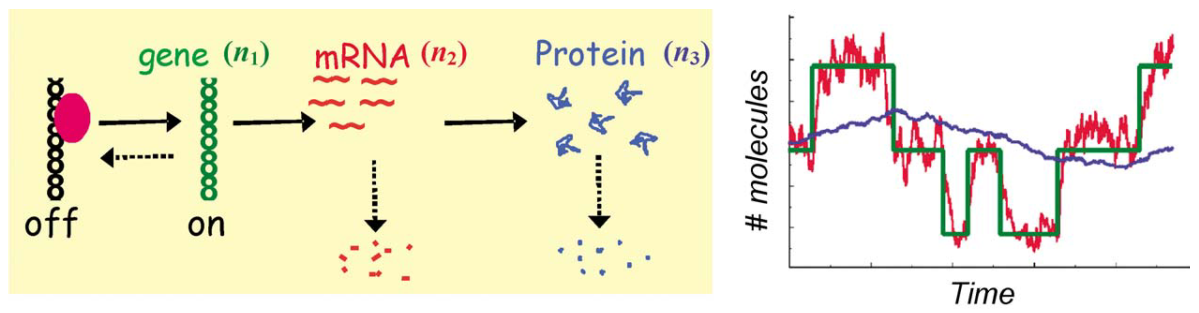
\includegraphics[width=0.9\textwidth]{fig/stochgeneexpdyn.png}\\
{\scriptsize
$n_1$ number of active genes, $n_2$ number of mRNAs, $n_3$ proteins per cell
\begin{align*}
\frac{d \langle n_1 \rangle}{dt} = &\lambda_1^+ (n_1^{max}-\langle n_1 \rangle -\lambda_1^- \langle n_1 \rangle\\
\frac{d \langle n_2 \rangle}{dt} = &\lambda_2 \langle n_1 \rangle -\langle n_2 \rangle / \tau_2\\
\frac{d \langle n_3 \rangle}{dt} = &\lambda_3 \langle n_2 \rangle - \langle n_3 \rangle / \tau_3
\end{align*}}
\end{center}
\end{frame}

%!TEX root = ../../beamer.tex
\begin{frame}
Birth-death process \hfill \cite{Erban2007}
{\scriptsize
\begin{align*}
A \xrightarrow{k_1} \varnothing\\
\varnothing \xrightarrow{k_2} A
\end{align*}}
%\vspace{1em}
\begin{center}
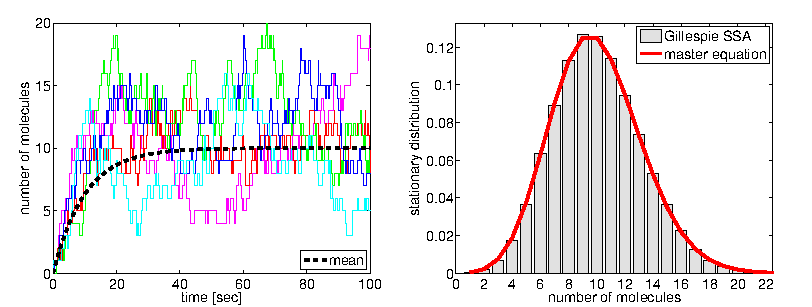
\includegraphics[width=0.9\textwidth]{fig/stochsimbirthdeathprocess.pdf}\\
\end{center}
{\scriptsize
\begin{align*}
\frac{dp_n}{dt}&=k_1(n+1)p_{n+1} - k_1 n p_n + k_2 p_{n-1} - k_2 p_n\\
\phi(n) &= \lim_{t\rightarrow\infty}p_n(t)\\
% 0 &= k_1 \phi(1) - k_2 \phi(0)\\
% 0 &= k_1(n+1)\phi(n+1) - k_1 n \phi(n) + k_2 \phi(n-1) - k_2 \phi(n)\\
\phi(1) &= \frac{k_2}{k_1} \phi(0)\\
\phi(n+1) &= \frac{1}{k_1(n+1)}\left[k_1 n \phi(n) - k_2 \phi(n-1) + k_2 \phi(n) \right]
\end{align*}}
\end{frame}

%!TEX root = ../../beamer.tex
\begin{frame}
\frametitle{stochastic bistability}
\begin{center}
{\scriptsize
$\varnothing \xrightleftharpoons[k_4]{k_3} A$ \hskip 1cm $2A \xrightleftharpoons[k_2]{k_1} 3A$\\
$\frac{d \langle A \rangle}{dt} = -k_2 \langle A \rangle^3 + k_1 \langle A \rangle^2 - k_4 \langle A \rangle + k_3$}
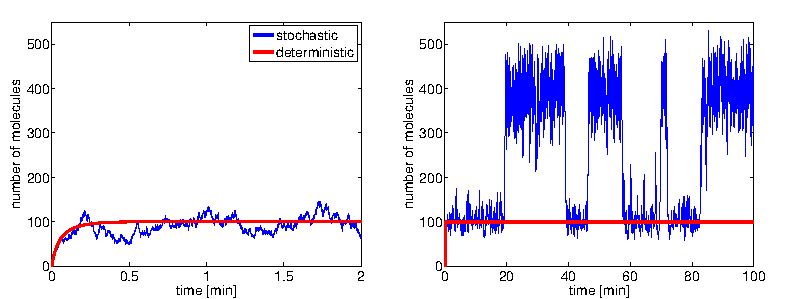
\includegraphics[width=0.9\textwidth]{fig/stochsimbistable.pdf}
\end{center}
\end{frame}

\begin{frame}
\vspace{1em}
\begin{center}
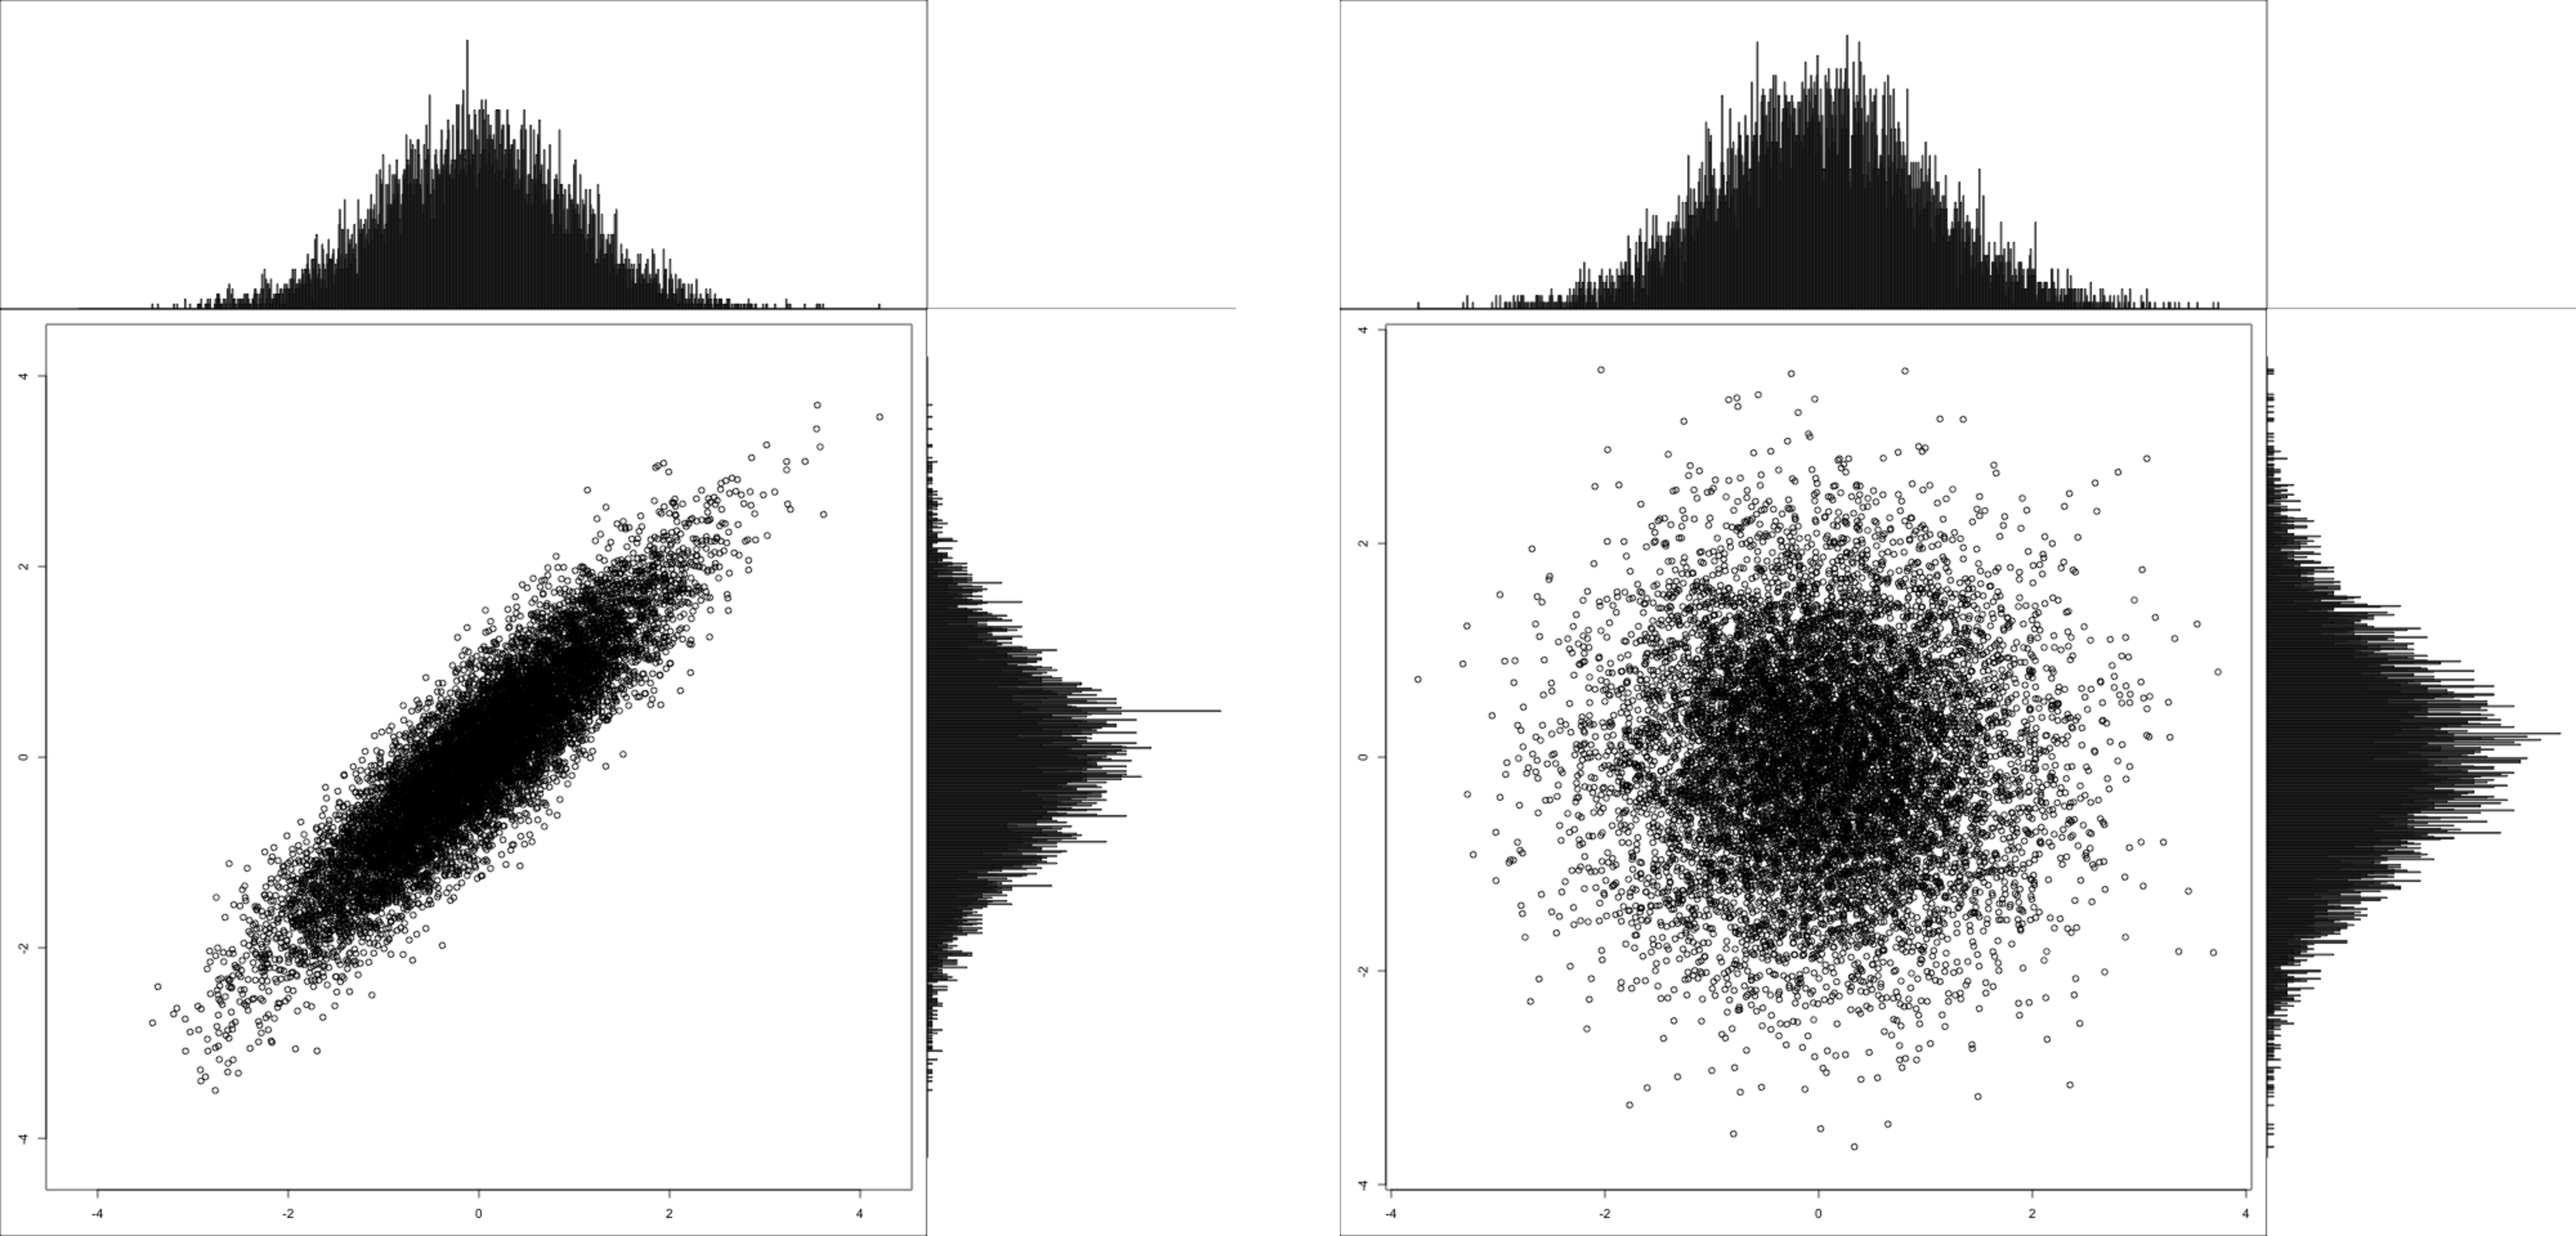
\includegraphics[width=0.8\textwidth]{fig/mvnormaltwo.pdf}\\
\end{center}
\end{frame}

\begin{frame}
\vspace{1em}
\frametitle{stochasticity in gene regulatory networks}
\begin{center}
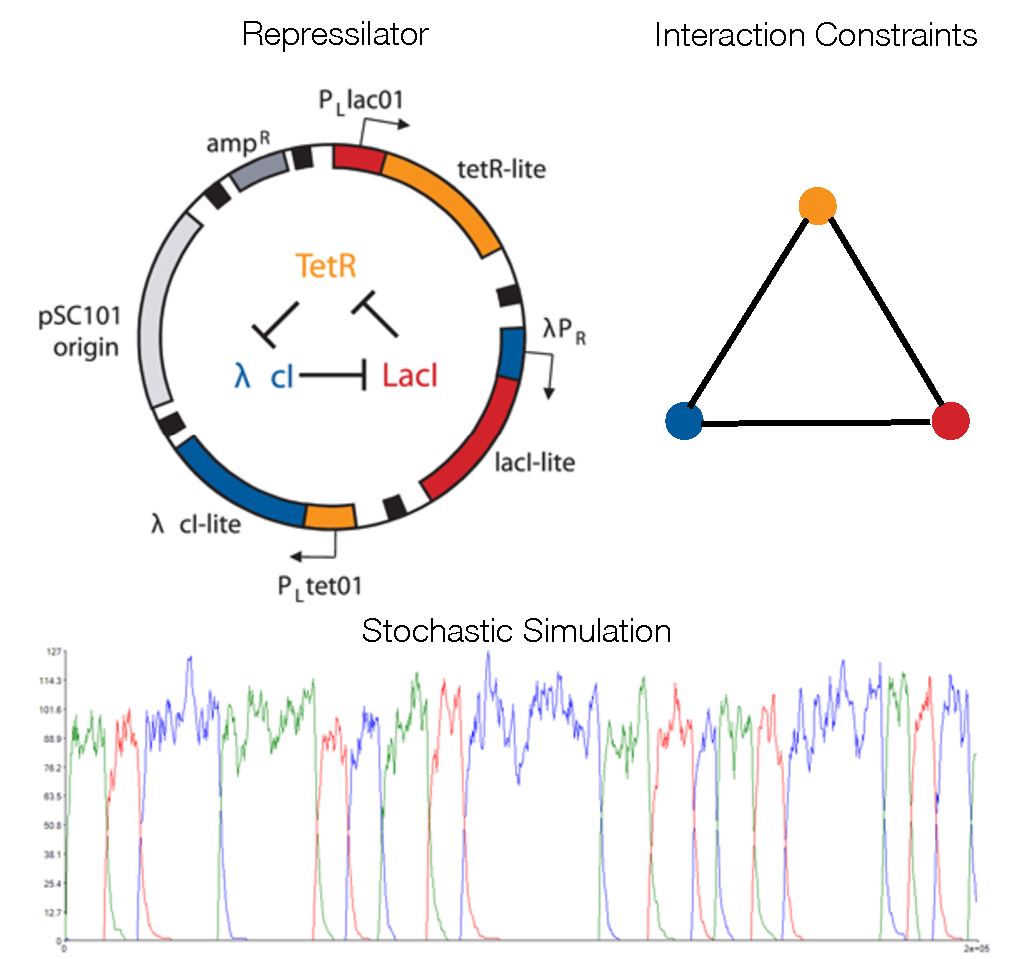
\includegraphics[width=0.6\textwidth]{fig/repressilator_constraints.pdf}\\
\hfill \cite{Elowitz2000b}
\end{center}
\end{frame}

%!TEX root = ../../beamer.tex
\begin{frame}
\vspace{1em}
\frametitle{stochastic dynamics in probability space}
\begin{center}

\includegraphics[width=0.8\textwidth]{fig/stochdynss.pdf}
\end{center}
\end{frame}

%\begin{frame}
\vspace{1em}
\begin{center}
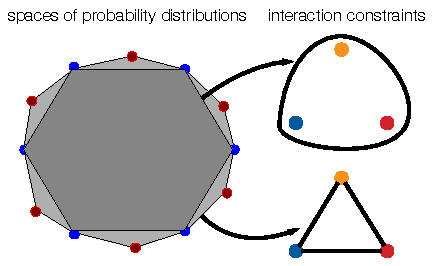
\includegraphics[width=0.7\textwidth]{fig/spacesandconstraints.pdf}\\
\end{center}
\end{frame}


%\begin{frame}
\begin{columns}[c]
\begin{column}{0.5\textwidth}
\begin{block}{\textbf{Observe gene expression}}
\begin{small}
\begin{itemize}
\item regardless of the structure of their interactions, \textbf{genes} can be indexed as $L = \{1, \ldots, l \}$
\item taking into account interactions, a \textbf{gene regulatory network module} is a subset of genes $O \subseteq L$ and these can be collected into a covering of the genotype space $\mathcal{G}$ where $L = \cup_{O \in \mathcal{G}} O$
\item regardless of the level of observation the total number of \textbf{phenotype values} under consideration can be indexed as $P = \{ 1, \ldots, p \} $
%\item an observation of a gene can take on different forms at different levels of "phenotypic" evaluation
\end{itemize}
\end{small}
\end{block}
\end{column}
\begin{column}{0.5\textwidth}
\begin{center}
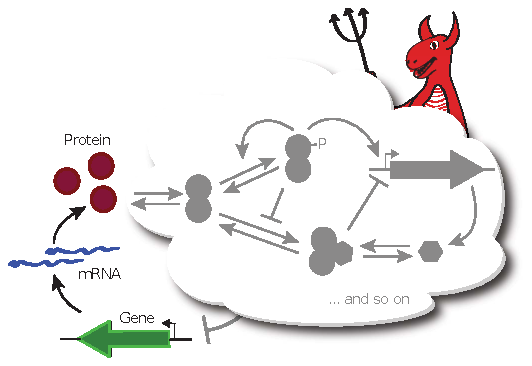
\includegraphics[width=0.8\textwidth]{fig/geneexpressiondemon.pdf}
\cite{Lestas2010}
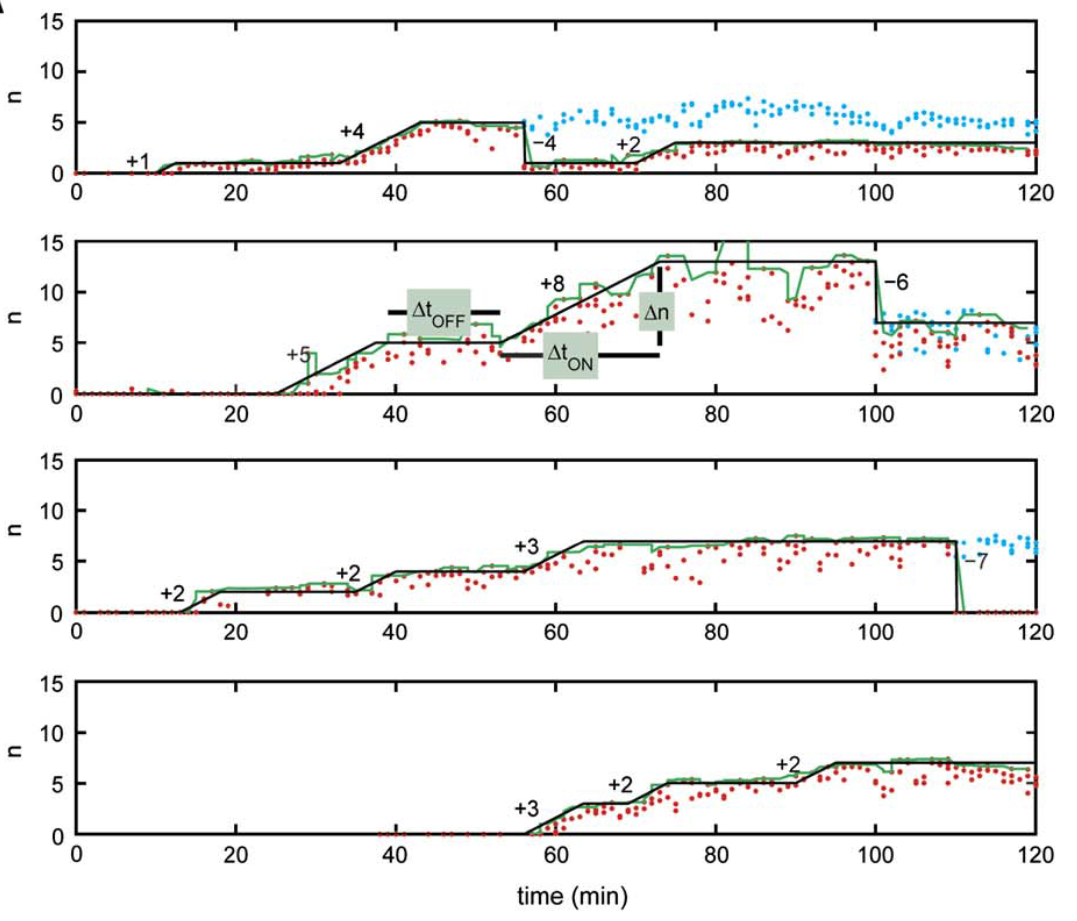
\includegraphics[width=0.8\textwidth]{fig/transcriptcounts.png}
\cite{Golding2005}
\end{center}
\end{column}
\end{columns}
\end{frame}

%\begin{frame}
\begin{columns}[c]
\begin{column}{0.5\textwidth}
\begin{block}{\textbf{Observe gene expression}}
\begin{itemize}
\item examples of phenotypes: \begin{small}
1) transcript counts derived from RNA-seq data 2) qualitative organismal phenotypic characteristics such as coat color in mice or wing shape in flies
\end{small}
\item regardless of the level of observation the total number of \textbf{phenotype values} under consideration can be indexed as $P = \{ 1, \ldots, p \} $
\end{itemize}
\end{block}
\end{column}
\begin{column}{0.5\textwidth}
\begin{center}
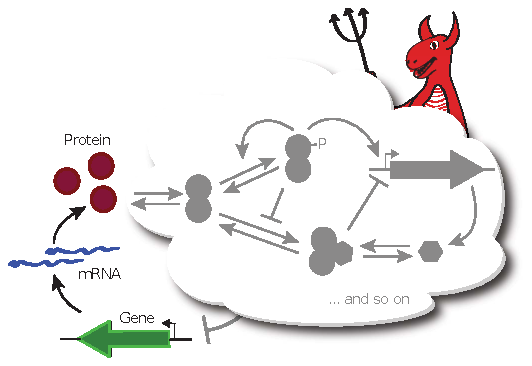
\includegraphics[width=1.0\textwidth]{fig/geneexpressiondemon.pdf}
\end{center}
\end{column}
\end{columns}
\end{frame}

%\begin{frame}
\begin{center}
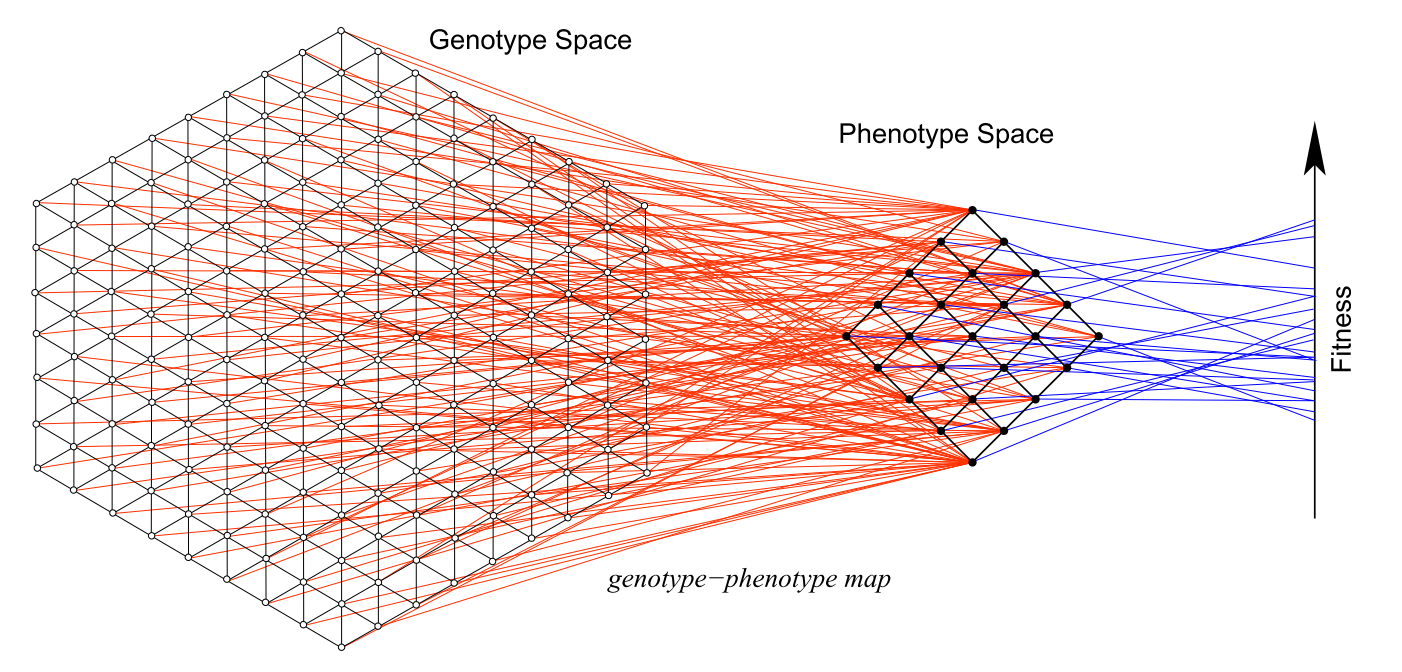
\includegraphics[width=0.8\textwidth]{fig/gpmap.png}\\
\hfill \cite{Stadler2002}
\end{center}
Simultaneous observation of the phenotype values of a subset $U \subseteq L$ of genes induces a genotype-phenotype mapping
$$
e \colon U \longrightarrow P
$$
\end{frame}

%\begin{frame}
%\begin{block}{\textbf{Concepts}}
\begin{center}
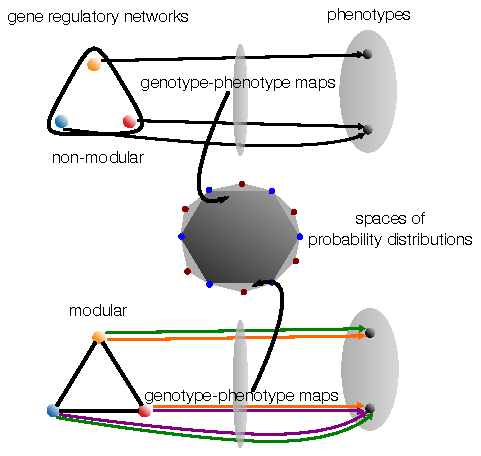
\includegraphics[width=0.8\textwidth]{fig/spacesconstraintsmaps.pdf}
\end{center}
%\end{block}
\end{frame}

